\subsubsection{Document formatting}
The tool also provides various document formatting options to pick from where these options are designed to help the user maintain a consistent formatting style throughout their document. The tool provides the following formatting options: brace location; indentation; comment style; punctuation; and object structure. All of these options make use of the abstract syntax tree (AST) that is generated for each document. The AST contains all information about the document in a programmatic way as provided by the Roslyn application programming interface (API). Navigating and interpreting the AST as necessary for each of the formatting options is needed.

\subsubsubsection{Comments}
Comments can be styled in various ways, the tool provides options to force comments to be on their own lines, or inline with code, and additionally choose wether comments should have a leading space or a trailing full stop. Each item in the AST contains a relative location to the document. Using this location span we can determine what line the comment is on. If the user has configured comments to be on a new line then we can navigate backwards through the AST to check if there are any non-whitespace tokens on the same line as the comment. If there are then we can insert a new line token before the comment and add any necessary indentation. We can make some minor performance improvements by not checking tokens after the comment as single-line comments defined by using the double backslash trivia will always be the last non-whitespace token a line.
Before styling comments, the tool will check to see if the comment token contains a mostly-text based comment or a commented out line of code, this is achieved by using a regex pattern on the token which captures words but not code. Following C\#'s syntax, a code comment is considered to be any comment that contains more camel case words with trailing punctuation than it does regular words. The regular expression pattern used, \texttt{(?<![.])\textbackslash b(?:[A-Z][a-z]*|[a-z]+| )\textbackslash b(?![.(][A-z])}, can be broken down as follows:
\begin{itemize}
    \item \texttt{(?<![.])} Don't capture when the text follows a full-stop.
    \item \texttt{\textbackslash b} Limit the search to be between word boundaries (i.e. is a letter followed by a non-letter).
    \item \texttt{(?:} Capture everything inside as a single match.
    \begin{itemize}
        \item \texttt{[A-Z][a-z]*} Capture a Capital and optinally unlimited lowercase letters, or...
        \item \texttt{[a-z]+} Capture one or more lowercase letters, or...
        \item Include spaces in the search captures.
    \end{itemize}
    \item \texttt{(?![.(][A-z])} Don't capture when the sequence ends with either a . or ( as these are common code tokens that often directly proceed text, so long as it is followed by another A-z character.
\end{itemize}

Within the user configuration file, an optional option can also be specified to set the sensitivity of the comment detection. By default this value is set to 50\% meaning that if the number of characters matched in the pattern is greater than 50\% of the total number of characters in the comment token string, it is to be considered a comment. If the result determines that the token is a code comment, the tool will not apply any formatting to the comment as it is assumed that the comment is a commented out line of code. Otherwise if the comment token is a mostly-text based comment, the tool will proceed to run additional checks on the token. The benefit to using a detection algorithm like this is that it works across human languages without the need for a dictionary of common words to be implemented, the downside however is that it may not always work if the text does not match the pre-defined pattern rules, though through testing it more often than not works as expected not producing false positives.

\subsubsubsection{Indentation}
To determine indentation levels for a given line the document is navigated line-by-line. A last-in-first-out (LIFO) stack is created to hold information about the current context level. A context level is determined by the following tokens: \texttt{\{ \} ( ) [ ]}. When a token is found that increases the context level the current context level is pushed onto the stack, and when a token is found that decreases the context level the stack is popped. The indentation level is then determined by the number of items in the stack multiplied by the user-defined indentation size. This method allows for the tool to determine the correct indentation level for each line in the document.
A simple text search for the tokens cannot be relied upon as they may be part of a string or comment, therefore we have to navigate the AST to find the tokens. Additionally, the indentation level cannot be properly be calculated if the stack contains an invalid sequence of tokens. For example, if the stack contains \texttt{\{ [ \}}, the indentation level cannot be calculated as the stack is in an invalid state. However, this should not occur as our custom analyzers are configured to only be run on syntactically valid C\# code which is determined by the compiler.

\subsubsubsection{Punctuation and brace location}

\begin{wrapfigure}{r}{0.275\textwidth}
    \centering
    \caption{YAML Configuration for Punctuation}
    \label{fig:YAMLPunctuation}
    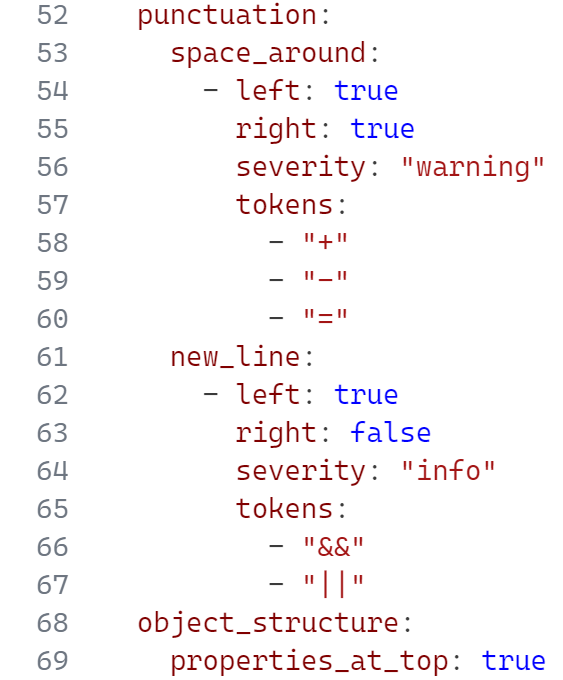
\includegraphics[width=0.275\textwidth]{Figures/YAMLConfigurationPunctuation.png}
\end{wrapfigure}

The punctuation sub-module allows the user to configure properties of language punctuation. In C\# punctuation is any token that is not a keyword or object variable, for example \texttt{; + -} etc. The punctuation sub-module allows the user to configure the spacing around punctuation, and wether punctuation should be on the same line as the previous token or on a new line. Within the YAML configuration file the user has the ability to define as many punctuation rules as they desire for the following options: space around, and new line. The tool will then navigate the AST to find any matching punctuation and adhere it to the configuration. For each of these options within the YAML file, the user should provide an array of configurations. Each of these configurations are to contain options for the formatter, a severity and a list of tokens that the rule should be applied to (see figure \ref{fig:YAMLPunctuation}).

The brace location works in a very similar way to the punctuation, however the brace location has to work slightly differently for the closing brace because the closing brace, if configured to be on a new line, must have 1 less indentation than what the tokens would otherwise have.

\subsubsubsection{Object structure}
The object structure sub-module is rather minimal but can have a major impact on code readability. It provides the user with the option to force object properties and fields to be at the top of the object declaration with all methods at the bottom. This has a huge impact on readability and debugging as it contributes significantly to reducing the amount of spaghetti code. Spaghetti code is code that is difficult to read and understand due to poor structure, which can be caused by having methods and properties mixed together in a class. By separating out the methods and properties it makes it far easier to understand what members a class has as there is no need to randomly dig through a class or struct to find potentially tucked away properties and fields between large method bodies.
As before the sub-module will traverse the abstract syntax tree and if any object declarations are encountered, a sub-loop will be run to check the order of the object members. If for example, a method declaration is found and further down the object declaration a property is found, the tool will create a diagnostic and return it to the user hinting that the object should be restructured. If the suggested change is accepted by the user the sub-module will move any methods to the bottom of the object declaration. During this operation various operations are made on the AST and with each subsequent modification a new AST is generated. This introduces a new problem of keeping track of other nodes that we may want to move. Fortunately the Roslyn API provides a way to keep track of the original node that was moved and from this we can track nodes that need to be moved, deleted or replaced without having to re-traverse the AST for similar matching nodes to those produced by the diagnostic from before.
